\documentclass{article}
\usepackage[T1]{fontenc}
\usepackage[polish]{babel}
\usepackage[utf8]{inputenc}
\usepackage{hyperref}
\usepackage{geometry}
 \geometry{
 a4paper,
 total={170mm,257mm},
 left=20mm,
 top=20mm,
 }
\usepackage{listings} 
\lstset{language=Python, 
        basicstyle=\ttfamily\small, 
        keywordstyle=\color{keywords},
        commentstyle=\color{comments},
        stringstyle=\color{red},
        showstringspaces=false,
        identifierstyle=\color{green},
        keywords=[2]{pow},
        frame = single,
        keywordstyle=[2]{\color{orange}},
} 
\usepackage{pdfpages}
\usepackage{xcolor}
\usepackage{graphicx}
\usepackage{fancyvrb}
\usepackage{amsfonts}
\usepackage{stmaryrd}
\usepackage{amsmath}
\usepackage{psfrag}
\usepackage{wrapfig}
\usepackage{framed, color}
\definecolor{shadecolor}{rgb}{1., 0.8, 0.3}
\newcommand{\hlc}[2][shadecolor]{ 	{\sethlcolor{#1} \hl{#2}} }
\usepackage{fancyvrb}
\graphicspath{ {./images/} }
\definecolor{keywords}{RGB}{255,0,90}
\definecolor{comments}{RGB}{0,0,113}
\definecolor{red}{RGB}{160,0,0}
\definecolor{green}{RGB}{0,150,0} 
\usepackage{enumitem}
\usepackage{fancyhdr}
\cfoot{Programowanie aplikacji sieciowych, część 1 | Katarzyna Mazur}
\renewcommand{\footrulewidth}{0.4pt}
\fancyfoot[LE,RO]{\thepage}
\pagestyle{fancy}
\setcounter{tocdepth}{3}
\setcounter{secnumdepth}{3}
\usepackage{color,soul}

\title{Programowanie aplikacji sieciowych \\ \small Zbiór zadań, część pierwsza}
\date{}
\author{Katarzyna Mazur}

\begin{document}

\maketitle
\newpage

\tableofcontents

\newpage

\section{Zadania wprowadzające}

\begin{enumerate}[label=\textbf{1.\arabic*}]\setlength{\itemsep}{1em}
    \item  Napisz program, w którym pobierzesz od użytkownika nazwę pliku tekstowego w formacie \texttt{*.txt}, a następnie skopiujesz go do pliku pod nazwą \texttt{lab1zad1.txt}. Zadbaj o prawidłową obsługę błędów.
    \item Napisz program, w którym pobierzesz od użytkownika nazwę pliku graficznego w formacie \texttt{*.png}, a następnie skopiujesz go do pliku pod nazwą \texttt{lab1zad2.png}. Zadbaj o prawidłową obsługę błędów.
    \item Napisz program, w którym pobierzesz od użytkownika adres \texttt{IPv4}, a następnie sprawdzisz, czy jest on prawidłowym adresem. Zadbaj o prawidłową obsługę błędów. \textit{Podpowiedź: zadanie możesz rozwiązać przy pomocy wyrażeń regularnych}
    \item Napisz program, w którym pobierzesz od użytkownika adres \texttt{IPv6}, a następnie sprawdzisz, czy jest on prawidłowym adresem.  Zadbaj o prawidłową obsługę błędów. \textit{Podpowiedź: zadanie możesz rozwiązać przy pomocy wyrażeń regularnych}
    \item Napisz program, który jako argument linii poleceń pobierze od użytkownika adres \texttt{IPv4}, a następnie wyświetli odpowiadającą mu nazwę \texttt{hostname} (nazwę domenową). Zadanie rozwiąż bez użycia dodatkowych bibliotek. Zadbaj o prawidłową obsługę błędów.
\end{enumerate}

\newpage 
\section{Analiza pakietów sieciowych}

\begin{enumerate}[label=\textbf{2.\arabic*}]\setlength{\itemsep}{1em}
    \item \label{ex21} Poniżej znajduje się pełny zapis datagramu UDP w postaci szesnastkowej. \\

\begin{figure}[h!t!p!]
\centering
\begin{BVerbatim}
ed 74 0b 55 00 24 ef fd 70 72 6f 67 72 61
6d 6d 69 6e 67 20 69 6e 20 70 79 74 68 6f 
6e 20 69 73 20 66 75 6e
\end{BVerbatim}
\end{figure}

\noindent  Wiedząc, że w zapisie szesnastkowym jedna cyfra reprezentuje $4$ bity, oraz znając strukturę datagramu UDP: 

\begin{figure}[ht!]
\centering
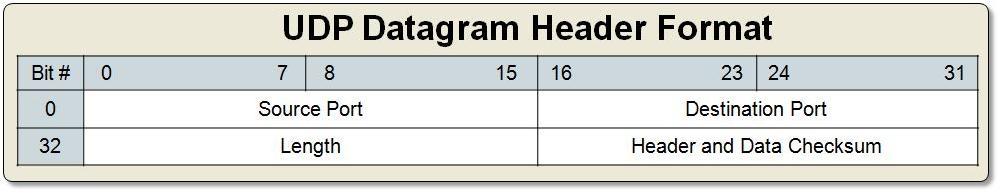
\includegraphics[scale=0.5]{/ch2/udp.jpg}
\end{figure}

\noindent Napisz program, który z powyższego datagramu UDP wydobędzie: 

\begin{itemize}
\item numer źródłowego portu
\item numer docelowego portu
\item dane (ile bajtów w tym pakiecie zajmują dane?)
\end{itemize}

\noindent A następnie uzyskany wynik w postaci: \hlc[shadecolor]{ zad2.1odp;src;X;dst;Y;data;Z } gdzie:

\begin{itemize}
\item X to wydobyty z pakietu numer portu źródłowego
\item Y to wydobyty z pakietu numer portu docelowego
\item Z to wydobyte z pakietu dane 
\end{itemize}

 prześle do serwera UDP działającego na wskazanym porcie pod podanym adresem IPv4, w celu sprawdzenia, czy udało się prawidłowo odczytać wymagane pola. Serwer zwróci odpowiedź \texttt{TAK} lub \texttt{NIE}, a w przypadku błędnego sformatowania wiadomości, odeśle odpowiedź \texttt{BAD\_SYNTAX}.  Zadanie rozwiąż bez użycia dodatkowych bibliotek (korzystaj jedynie z gniazd). Zadbaj o prawidłową obsługę błędów. 

 % ####################################################################################################################  
  \item Zmodyfikuj program z zadania \ref{ex21} w taki sposób,  aby łączył się z serwerem posiadającym adres IPv6.  Adres IPv6 serwera i numer portu pobierz jako argumenty linii poleceń. Zadanie rozwiąż bez użycia dodatkowych bibliotek (korzystaj jedynie z gniazd). Zadbaj o prawidłową obsługę błędów. 
 

% ####################################################################################################################  
 \item \label{ex22} Poniżej znajduje się pełny zapis segmentu TCP w postaci szesnastkowej (pole opcji ma 12 bajtów). \\ 

\begin{figure}[h!t!p!]
\centering
\begin{BVerbatim}
0b 54 89 8b 1f 9a 18 ec bb b1 64 f2 80 18
00 e3 67 71 00 00 01 01 08 0a 02 c1 a4 ee 
00 1a 4c ee 68 65 6c 6c 6f 20 3a 29
\end{BVerbatim}
\end{figure}\mbox{}

\noindent  Wiedząc, że w zapisie szesnastkowym jedna cyfra reprezentuje $4$ bity, oraz znając strukturę segmentu TCP:\\

\begin{figure}[ht!]
\centering
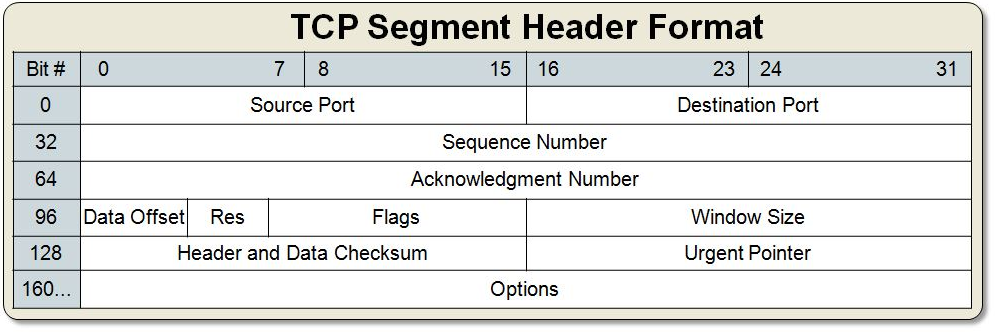
\includegraphics[scale=0.45]{./ch2/tcp.png}
\end{figure}
\newpage 
\noindent Napisz program, który z powyższego segmentu TCP wydobędzie: 

\begin{itemize}
\item numer źródłowego portu
\item numer docelowego portu
\item dane (ile bajtów w tym pakiecie zajmują dane?)
\end{itemize}

\noindent A następnie uzyskany wynik w postaci: \hlc[shadecolor]{ zad2.3odp;src;X;dst;Y;data;Z } gdzie:

\begin{itemize}
\item X to wydobyty z pakietu numer portu źródłowego
\item Y to wydobyty z pakietu numer portu docelowego
\item Z to wydobyte z pakietu dane 
\end{itemize}

 prześle do serwera TCP działającego na wskazanym porcie pod podanym adresem IPv4, w celu sprawdzenia, czy udało się prawidłowo odczytać wymagane pola. Serwer zwróci odpowiedź \texttt{TAK} lub \texttt{NIE}, a w przypadku błędnego sformatowania wiadomości, odeśle odpowiedź \texttt{BAD\_SYNTAX}.  Zadanie rozwiąż bez użycia dodatkowych bibliotek (korzystaj jedynie z gniazd). Zadbaj o prawidłową obsługę błędów. 
% ####################################################################################################################  
 

  \item Zmodyfikuj program z zadania \ref{ex22} w taki sposób,  aby łączył się z serwerem posiadającym adres IPv6.  Adres IPv6 serwera i numer portu pobierz jako argumenty linii poleceń. Zadanie rozwiąż bez użycia dodatkowych bibliotek (korzystaj jedynie z gniazd). Zadbaj o prawidłową obsługę błędów. 

\end{enumerate}

\newpage
\section{Gniazda klienckie}

\subsection*{Gniazda TCP}

\begin{enumerate}[label=\textbf{3.\arabic*}]\setlength{\itemsep}{1em}
    \item \label{ex31} Napisz program klienta, w którym połączysz się z serwerem na danym porcie przy użyciu protokołu TCP. Adres IPv4 serwera i numer portu pobierz jako argumenty linii poleceń. Wyświetl informację, czy udało się nawiązać połączenie. Program powinien akceptować adres w postaci adresu IPv4 jak i hostname. Zadanie rozwiąż bez użycia dodatkowych bibliotek (korzystaj jedynie z gniazd). Zadbaj o prawidłową obsługę błędów. 
    
    \item Zmodyfikuj program z zadania \ref{ex31} w taki sposób, aby łączył się z serwerem posiadającym adres IPv6.  Adres IPv6 serwera i numer portu pobierz jako argumenty linii poleceń. Zadanie rozwiąż bez użycia dodatkowych bibliotek (korzystaj jedynie z gniazd). Zadbaj o prawidłową obsługę błędów. 
    
    \item \label{ex33} Napisz program klienta (prosty skaner portów sieciowych), który dla danego serwera przy użyciu protokołu TCP będzie sprawdzał, jakie porty są otwarte, a jakie zamknięte. Adres IPv4 serwera pobierz jako argument linii poleceń. Program powinien akceptować adres w postaci adresu IPv4 jak i hostname.  Zadanie rozwiąż bez użycia dodatkowych bibliotek (korzystaj jedynie z gniazd). Zadbaj o prawidłową obsługę błędów. 
    
    \item  Zmodyfikuj program z zadania \ref{ex33} w taki sposób,  aby łączył się z serwerem posiadającym adres IPv6.  Adres IPv6 serwera i numer portu pobierz jako argumenty linii poleceń. Zadanie rozwiąż bez użycia dodatkowych bibliotek (korzystaj jedynie z gniazd). Zadbaj o prawidłową obsługę błędów. 
    
    \item \label{ex35} Napisz program klienta, który z serwera o podanym adresie IPv4 i porcie pobierze aktualną datę i czas, a następnie wyświetli je na konsoli.  Adres IPv4 serwera i numer portu pobierz jako argumenty linii poleceń. Zadanie rozwiąż bez użycia dodatkowych bibliotek (korzystaj jedynie z gniazd). Zadbaj o prawidłową obsługę błędów. 
    
     \item Zmodyfikuj program z zadania \ref{ex35} w taki sposób,  aby łączył się z serwerem posiadającym adres IPv6.  Adres IPv6 serwera i numer portu pobierz jako argumenty linii poleceń. Zadanie rozwiąż bez użycia dodatkowych bibliotek (korzystaj jedynie z gniazd). Zadbaj o prawidłową obsługę błędów. 
     
     \item \label{ex37} Napisz program klienta, który połączy się z serwerem TCP działającym pod podanym adresem IPv4 na podanym porcie, a następnie wyśle do niego wiadomość i odbierze odpowiedź.  Adres IPv4 serwera i numer portu pobierz jako argumenty linii poleceń. Zadanie rozwiąż bez użycia dodatkowych bibliotek (korzystaj jedynie z gniazd). Zadbaj o prawidłową obsługę błędów. 
     
     \item Zmodyfikuj program z zadania \ref{ex37} w taki sposób,  aby łączył się z serwerem posiadającym adres IPv6.  Adres IPv6 serwera i numer portu pobierz jako argumenty linii poleceń. Zadanie rozwiąż bez użycia dodatkowych bibliotek (korzystaj jedynie z gniazd). Zadbaj o prawidłową obsługę błędów. 
     
     \item \label{ex39} Napisz program klienta, który połączy się z serwerem TCP działającym pod podanym adresem IPv4 na podanym porcie,  a następnie będzie w pętli wysyłał do niego tekst wczytany od użytkownika (jako argument wywołania programu bądź jako dane podawane na konsoli), i odbierał odpowiedzi.  Adres IPv4 serwera i numer portu pobierz jako argumenty linii poleceń. Zadanie rozwiąż bez użycia dodatkowych bibliotek (korzystaj jedynie z gniazd). Zadbaj o prawidłową obsługę błędów. 
     
     \item Zmodyfikuj program z zadania \ref{ex39} w taki sposób,  aby łączył się z serwerem posiadającym adres IPv6.  Adres IPv6 serwera i numer portu pobierz jako argumenty linii poleceń. Zadanie rozwiąż bez użycia dodatkowych bibliotek (korzystaj jedynie z gniazd). Zadbaj o prawidłową obsługę błędów. 

    \item  \label{ex311} Napisz program klienta (prosty skaner portów sieciowych), który dla danego serwera przy użyciu protokołu TCP będzie sprawdzał, jakie porty są otwarte, a jakie zamknięte. Oprócz informacji o otwartych / zamkniętych portach, program powinien również wyświetlać informację o tym, jaka usługa jest uruchomiona na danym porcie (baner usługi).  Adres IPv4 serwera pobierz jako argument linii poleceń. Program powinien akceptować adres w postaci adresu IPv4 jak i hostname.  Zadanie rozwiąż bez użycia dodatkowych bibliotek (korzystaj jedynie z gniazd). Zadbaj o prawidłową obsługę błędów.  
    
    \item Zmodyfikuj program z zadania \ref{ex311} w taki sposób,  aby łączył się z serwerem posiadającym adres IPv6. Zadanie rozwiąż bez użycia dodatkowych bibliotek (korzystaj jedynie z gniazd). Zadbaj o prawidłową obsługę błędów. 
    
    \item \label{ex313} Napisz program klienta, który połączy się z serwerem TCP działającym pod podanym adresem IPv4 na podanym porcie, a następnie wyśle do niego wiadomość i odbierze odpowiedź. Warunkiem zadania jest, aby klient wysłał i odebrał od serwera wiadomość o maksymalnej długości 20 znaków. Zadanie rozwiąż bez użycia dodatkowych bibliotek (korzystaj jedynie z gniazd). Zadbaj o prawidłową obsługę błędów.  Uwzględnij sytuacje, gdy:
    \begin{itemize}
    \item wiadomość do wysłania jest za krótka - ma być wówczas uzupełniania do 20 znaków znakami spacji
    \item wiadomość do wysłania jest za długa - ma być przycięta do 20 znaków (lub wysłana w całości - sprawdź, co się wówczas stanie)
    \end{itemize}
    
    \item Zmodyfikuj program z zadania \ref{ex313} w taki sposób,  aby łączył się z serwerem posiadającym adres IPv6. Zadanie rozwiąż bez użycia dodatkowych bibliotek (korzystaj jedynie z gniazd). Zadbaj o prawidłową obsługę błędów. 
    
    \item \label{ex315} Dostępne dla gniazd funkcje \texttt{recv} i \texttt{send} nie gwarantują wysłania / odbioru wszystkich danych. Rozważmy funkcję \texttt{recv}. Przykładowo, $100$ bajtów może zostać wysłane jako grupa po $10$ bajtów, albo od razu w całości. Oznacza to, iż jeśli używamy gniazd TCP, musimy odbierać dane, dopóki nie mamy pewności, że odebraliśmy odpowiednią ich ilość. Napisz program klienta, który połączy się z serwerem TCP działającym pod podanym adresem IPv4 na podanym porcie, a następnie wyśle do niego wiadomość i odbierze odpowiedź. Dane odbieraj / wysyłaj w ten sposób, aby mieć pewność, że klient w rzeczywistości odebrał / wysłał wiadomość o wymaganej długości. Zadanie rozwiąż bez użycia dodatkowych bibliotek (korzystaj jedynie z gniazd). Zadbaj o prawidłową obsługę błędów. 
    
    \item Zmodyfikuj program z zadania \ref{ex315} w taki sposób,  aby łączył się z serwerem posiadającym adres IPv6. Zadanie rozwiąż bez użycia dodatkowych bibliotek (korzystaj jedynie z gniazd). Zadbaj o prawidłową obsługę błędów. 
   
\end{enumerate}

\subsection*{Gniazda UDP}

\begin{enumerate}[label=\textbf{3.\arabic*}, resume]\setlength{\itemsep}{1em}

\item \label{ex317}  Napisz program klienta, który połączy się z serwerem UDP działającym pod podanym adresem IPv4 na podanym porcie, a następnie wyśle do niego wiadomość i odbierze odpowiedź. Adres IPv4 serwera oraz numer portu pobierz jako argumenty linii poleceń. Program powinien akceptować adres w postaci adresu IPv4 jak i hostname.  Zadanie rozwiąż bez użycia dodatkowych bibliotek (korzystaj jedynie z gniazd). Zadbaj o prawidłową obsługę błędów.  

\item  Zmodyfikuj program z zadania \ref{ex317} w taki sposób,  aby łączył się z serwerem posiadającym adres IPv6.  Adres IPv6 serwera i numer portu pobierz jako argumenty linii poleceń. Zadanie rozwiąż bez użycia dodatkowych bibliotek (korzystaj jedynie z gniazd). Zadbaj o prawidłową obsługę błędów. 

\item \label{ex319} Napisz program klienta, który połączy się z serwerem UDP działającym pod podanym adresem IPv4 na podanym porcie,  a następnie będzie w pętli wysyłał do niego tekst wczytany od użytkownika, i odbierał odpowiedzi.    Adres IPv4 serwera i numer portu pobierz jako argumenty linii poleceń. Zadanie rozwiąż bez użycia dodatkowych bibliotek (korzystaj jedynie z gniazd). Zadbaj o prawidłową obsługę błędów. 

\item  Zmodyfikuj program z zadania \ref{ex319} w taki sposób,  aby łączył się z serwerem posiadającym adres IPv6. Adres IPv6 serwera i numer portu pobierz jako argumenty linii poleceń. Zadanie rozwiąż bez użycia dodatkowych bibliotek (korzystaj jedynie z gniazd). Zadbaj o prawidłową obsługę błędów. 

\item \label{ex321} Napisz program klienta, który połączy się z serwerem UDP działającym pod podanym adresem IPv4 na podanym porcie, a następnie prześle do serwera liczbę, operator, liczbę (pobrane od użytkownika) i odbierze odpowiedź. Adres IPv4 serwera i numer portu pobierz jako argumenty linii poleceń.  Zadanie rozwiąż bez użycia dodatkowych bibliotek (korzystaj jedynie z gniazd). Zadbaj o prawidłową obsługę błędów. 

\item  Zmodyfikuj program z zadania \ref{ex321} w taki sposób,  aby łączył się z serwerem posiadającym adres IPv6. Adres IPv6 serwera i numer portu pobierz jako argumenty linii poleceń. Zadanie rozwiąż bez użycia dodatkowych bibliotek (korzystaj jedynie z gniazd). Zadbaj o prawidłową obsługę błędów. 

\item \label{ex322} Napisz program klienta, który połączy się z serwerem UDP działającym pod podanym adresem IPv4 na podanym porcie, a następnie prześle do serwera pobrany z linii poleceń adres IP, i odbierze odpowiadającą mu nazwę hostname. Zadanie rozwiąż bez użycia dodatkowych bibliotek (korzystaj jedynie z gniazd). Zadbaj o prawidłową obsługę błędów. 

\item  Zmodyfikuj program z zadania \ref{ex322} w taki sposób,  aby łączył się z serwerem posiadającym adres IPv6. Adres IPv6 serwera i numer portu pobierz jako argumenty linii poleceń. Zadanie rozwiąż bez użycia dodatkowych bibliotek (korzystaj jedynie z gniazd). Zadbaj o prawidłową obsługę błędów. 

\item \label{ex323} Napisz program klienta, który połączy się z serwerem UDP działającym pod podanym adresem IPv4 na podanym porcie, a następnie prześle do serwera nazwę hostname pobraną z linii poleceń, i odbierze odpowiadający mu adres IP.  Zadanie rozwiąż bez użycia dodatkowych bibliotek (korzystaj jedynie z gniazd). Zadbaj o prawidłową obsługę błędów. 

\item Zmodyfikuj program z zadania \ref{ex323} w taki sposób,  aby łączył się z serwerem posiadającym adres IPv6. Adres IPv6 serwera i numer portu pobierz jako argumenty linii poleceń. Zadanie rozwiąż bez użycia dodatkowych bibliotek (korzystaj jedynie z gniazd). Zadbaj o prawidłową obsługę błędów. 
\end{enumerate}

\newpage
\section{Gniazda serwerowe}

\subsection*{Gniazda TCP}
\subsection*{Gniazda UDP}

\section{Protokoły pocztowe}
\subsection{Protokół SMTP}
\subsection{Protokół POP3}
\subsection{Protokół IMAP}

\section{Protokół HTTP}


\end{document}